\documentclass[a4paper]{article}
\usepackage{a4}
\usepackage{fancyhdr}
\usepackage[latin1]{inputenc}
\usepackage{mathpazo}

\usepackage{hyperref}
\hypersetup{pdfauthor={Georg Hennig},
	pdftitle={GIMP plugin astronomy},
	pdfsubject={},
	pdfproducer={LaTeX},
	linkcolor=green, %% for links on same page
	urlcolor=blue, %% links to URLs
	breaklinks=true, %% allow links to break across lines!
	colorlinks=false, %% obviously inverted logic :-(
	citebordercolor=0 0.5 0, %% color for \cite
	filebordercolor=0 0.5 0,
	linkbordercolor=0.5 0 0,
	menubordercolor=0.5 0 0,
	urlbordercolor=0 0.5 0.5,
	pdfborder=0 0 0, %% to show _really_ only a box around the links and not a filled recangle
	bookmarksopen=false,
	bookmarksnumbered=true,
	pdfstartview=FitH
}

% math
\usepackage{amssymb, graphicx}
\usepackage[intlimits]{amsmath}
\usepackage{booktabs}
\usepackage{nicefrac}
\usepackage{units}

% tabular / graphics
\usepackage{tabularx}
\usepackage{graphicx}
\usepackage{epsfig}
\usepackage{color}
\usepackage{xcolor}
\usepackage{picins}
\usepackage[justification=raggedright]{caption}
\usepackage{rotating}

\usepackage{palatino, url, multicol}

\renewcommand{\figurename}{Abb.}
\renewcommand{\tablename}{Tab.}

\title{GIMP plugin astronomy 0.8}
\author{Georg Hennig \\ \emph{georg.hennig@web.de}}

\begin{document}

\maketitle

\newpage

\tableofcontents

\newpage

\section{Installation}

\subsection{Compile}

\subsubsection{Unix}

Usually, it is enough to run
\begin{verbatim}
tar -xvjf gimp-plugin-astronomy-VERSION.tar.bz2
cd gimp-plugin-astronomy-VERSION
./configure --prefix=/usr
make
su
<your root password>
make install
\end{verbatim}

You can also skip the \emph{make install} part, and copy the plugins (manually) to the
\begin{verbatim}~/.gimp-2.4/plug-ins\end{verbatim}
folder, and the scripts to the
\begin{verbatim}~/.gimp-2.4/scripts\end{verbatim}
folder.

GIMP plugin astronomy requires the development packages of GIMP and Gtk+ and their dependencies,
and additionally the development packages of \emph{fftw} (Fastest Fourier Transform in the West, version 3, \url{http://www.fftw.org}) and \emph{GSL} (GNU scientific library, \url{http://www.gnu.org/software/gsl/}).
Often these packages are called \emph{gimp-VERSION-dev}, \emph{gsl-VERSION-dev}. Of course, you'll need a C development environment, which means \emph{make} and \emph{gcc} plus dependencies like \emph{gtk*-dev}, \emph{glib*-dev}, etc.

\subsubsection{Windows}

For building GIMP plugin astronomy for Windows (using MinGW), you need
\begin{itemize}
\item A working \emph{MinGW compiler}
\item \emph{make}
\item \emph{GIMP} development environment (headers and libraries), including its dependencies
\item \emph{GSL} library. You can compile it yourself, for example with these settings:
\begin{verbatim}
CFLAGS="-D_X86_=1 -Dtry=__try -Dexcept=__except -DWIN32 -D_WIN32
        -DGSL_DLL -DDLL_EXPORT -O3 -W -Wall -I.. -I../cblas"
LDFLAGS="-mwindows"
\end{verbatim}
\item \emph{FFTW}, version 3. (\emph{libfftw3-3.dll} and \emph{fftw3.h})
\end{itemize}


\subsection{Windows binaries}

To install gimp-plugin-astronomy on Windows systems, copy all files in the folder \emph{plugins} (all \emph{astronomy-*.exe} and \emph{*.dll} files) to
\begin{verbatim}c:\Documents and Settings\<User>\.gimp-2.4\plugins\end{verbatim}
and all files inside \emph{scripts} (all \emph{*.scm} files) to
\begin{verbatim}c:\Documents and Settings\<User>\.gimp-2.4\scripts\end{verbatim}
To have translated messages, copy the folder \emph{lib} into
\begin{verbatim}c:\Documents and Settings\<User>\.gimp-2.4\plugins\end{verbatim}
If building from sources, copy the file \emph{language.gmo} to
\begin{verbatim}lib/.../locale/<language>/LC_MESSAGES/gimp-plugin-astronomy.mo\end{verbatim}
The plugins are available in the GIMP image window under \emph{Filters $\rightarrow$ Astronomy $\rightarrow$ plugin name}.

\newpage

\section{Scripts}

\subsection{Background gradient batch}

To batch normalize the background of all images in a folder.
Run on the command line something like
\begin{verbatim}
gimp -i -b '(background-gradient-batch "*.jpg" 200 200 2 1.0 200 0 0)'
  -b '(gimp-quit 0)'
\end{verbatim}
Parameters are: image list, box width, box height, numbers of iteration of sigma clipping, sigma, minimum number of values inside a box, weighted values (0=all values,1=darkest,2=brightest), percentage of darkest or brightest values.
Look at background gradient plugin description below to see, what these settings mean.

\subsection{Brightness contrast batch}

This script sets brightness and contrast to all layers; it doesn't provide a preview as the normal brightness and contrast plugin.

\subsection{Set mode batch}

A simple batch script to set overlay mode to all layers.

\subsection{Border information}

Draws a border (up to 2 different colors) around your images and on the bottom some information about your image, up to 2 lines at up to 3 positions (aligned left, right and centered). \\
Example: \\
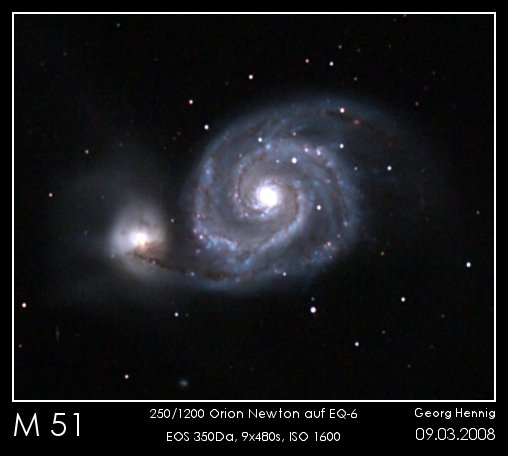
\includegraphics[width=0.7\textwidth]{border_information.jpg}


\subsection{Dark subtraction}

Subtracts a dark frame from all layers; naturally the dark frame should have the same size as all layers.

\subsection{Flat division}

Divides all layers by a flat field; size issue as above.

\subsection{Normalize batch}

Batch applies the normalize function (\emph{Layer $\rightarrow$ Colors $\rightarrow$ Automatic $\rightarrow$ Normlize}) to all layers.

\newpage

\section{Plug-ins}

\subsection{Align}

\begin{center}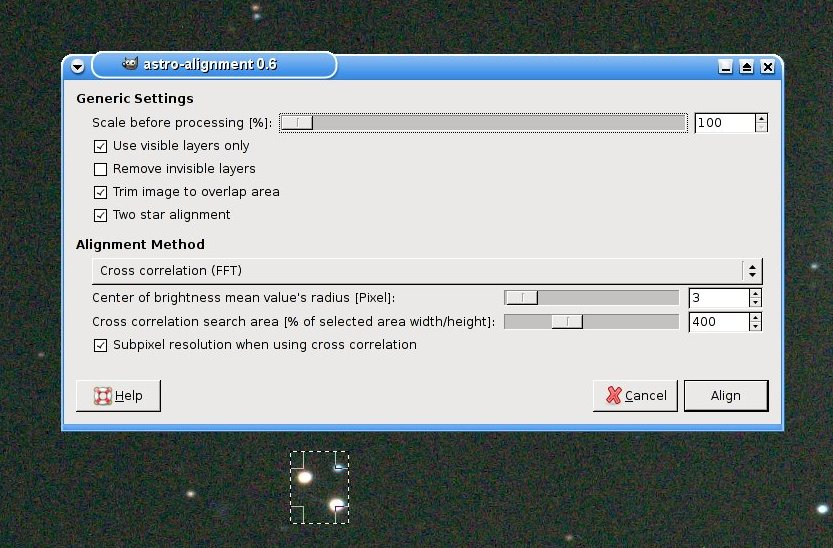
\includegraphics[width=1.0\textwidth]{align.jpg}\end{center}

% \subsubsection{Usage}
% 
% \subsubsection{Explanation}

This plug-in moves (and rotates) the layers that they overlap correctly. For alignment by center of disk / brightness, select the area, where the star is, that you want to user for alignment. For cross correlation alignment, select the object you want to use for selection (from the first layer). Optionally you can crop the image to the area, where the layers overlap. De-rotation is done by selecting a second star during alignment process.

\subsection{Artificial galaxy}

\begin{center}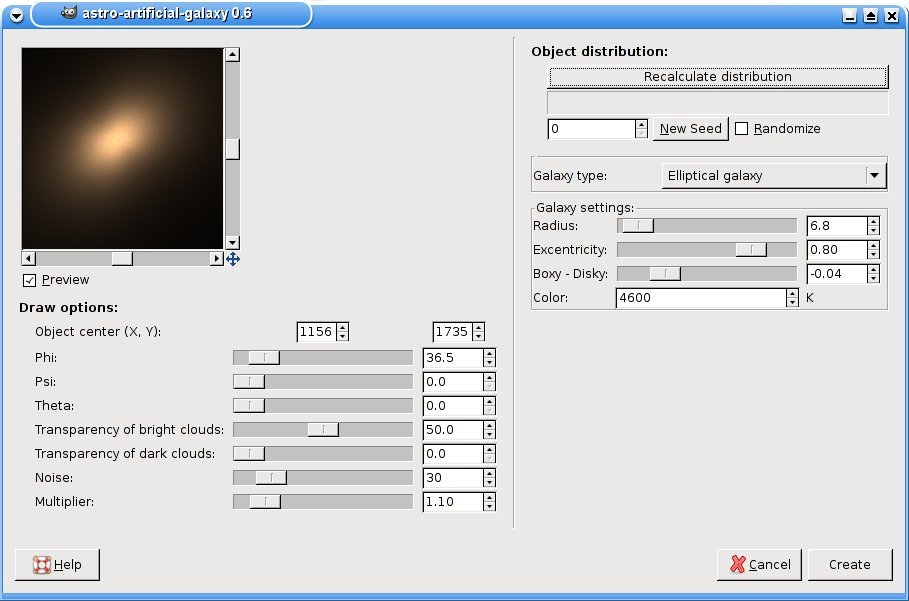
\includegraphics[width=1.0\textwidth]{artificial_galaxy.jpg}\end{center}

\subsubsection{Usage}

Creates an artificial galaxy.

\subsubsection{Explanation}

Quite difficult to implement, only elliptical galaxies by now.

\subsection{Artificial stars}

\begin{center}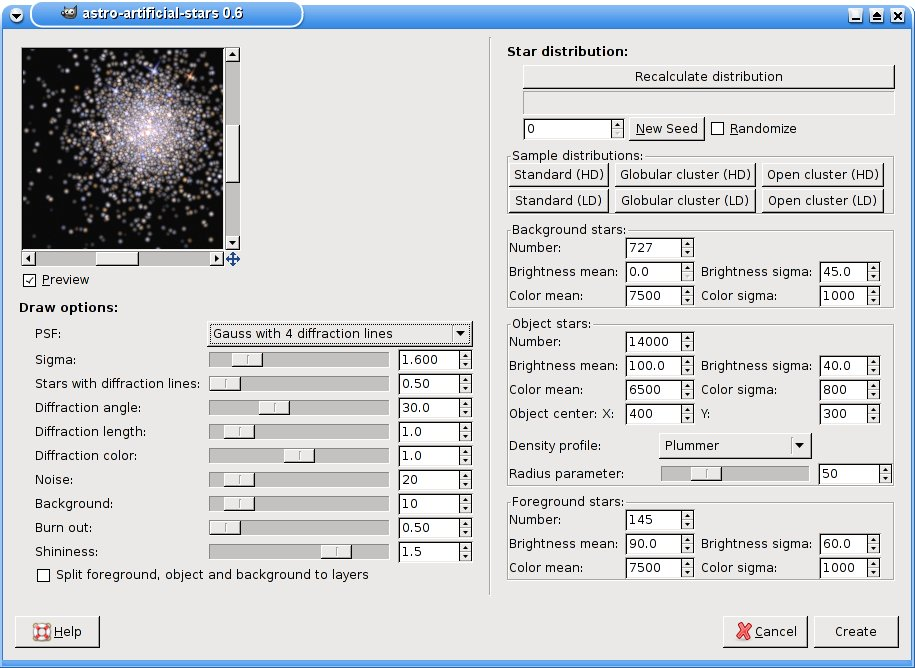
\includegraphics[width=1.0\textwidth]{artificial_stars.jpg}\end{center}
% 
% \subsubsection{Usage}
% 
% \subsubsection{Explanation}

Creates an artificial star distribution.
The interface is splitted: On the right side, you can set up the options for the star distribution, on the right side how they will be drawn. To actually calculate a star distribution, you need to click on the button, as recalculation might take very long for many stars.
Changes on the left side only affect the preview.
The sample distribution buttons give you an idea, what you can do with this plug-in.

\subsection{Background gradient}

\begin{center}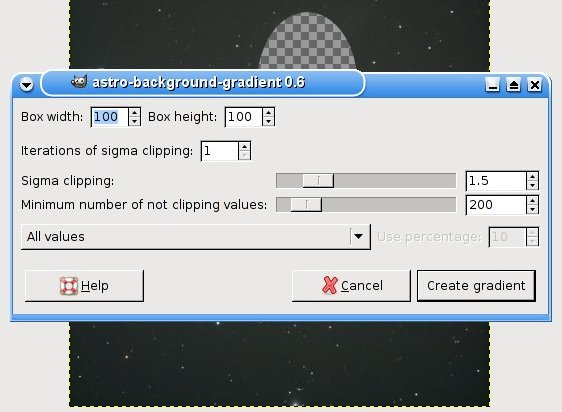
\includegraphics[width=0.6\textwidth]{background_gradient.jpg}\end{center}

\subsubsection{Usage}

This plugin fills a layer with the normalized background of a layer, described by a polynomial of 4th order.
To receive good results, copy your layer, cut out parts of the layer containing large objects with a color different than the background color (for example galaxies or nebulae) and then run the background gradient plugin on it.
The background gradient layer is set to ''divide'', as this will remove the background gradient by amplifying dark parts.
Of course, this will amplify noise, too.

\subsubsection{Explanation}

First, the plugin divides the layer into boxes with width and height defined by the user. The boxes at the edges can be smaller, depending on the layer and the box sizes.
Then it loops through all these boxes.

For each box, all pixel values (colors are treated seperately!) are sorted (pixels with alpha channel 0 are omitted).
If the user decided to consider only darkest (brightest) $z$ percent values, all other values are thrown away.
Then, the median and the standard deviation $\sigma$ of the remaining values is calculated.
If sigma clipping iteration is $c > 1$, all values $> \mathrm{median} + n \cdot \sigma$ and $< \mathrm{median} - n \cdot \sigma$ are thrown away and this step is repeated $c-1$ times.

Finally, if the number of remaining pixel values is big enough (compared to the minimum number requested by user), the arithmetic mean of the remaining values is calculated.

As this is done for each box, we have many mean pixel values, one at the position of each box.
These mean pixel values are the pivotal points for a linear regression fit to a polynomial of 4th order.

Then the absolute maximum of the polynomial is calculated, and normalized values are written to the background gradient layer (maximum corresponds to 255).

\subsection{Merge}

\begin{center}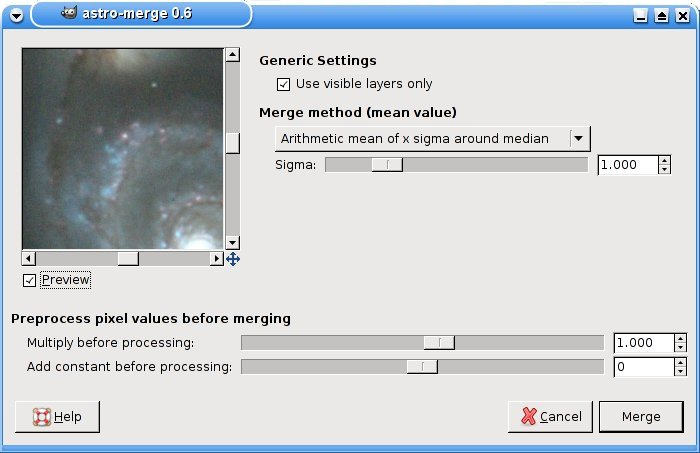
\includegraphics[width=0.8\textwidth]{merge.jpg}\end{center}

\subsubsection{Usage}
Calculates the mean value of overlapping layers and saves it into a new image.
You can choose, which method for the mean value you want: Arithmetic or geometric mean value, median, median / arithmetic mean or sigma median (1 or 2 passes).
Each pixel value can be modified by a multiplier and an additive constant.
For an explanation, what these settings mean, look below.

\subsubsection{Explanation}

First, this plugin resizes all layers to the image size (invisible to user).
This can lead to invisible areas (alpha channel is $0$) in a layer, where the layers don't overlap, except for layers without alpha channel: the areas won't be invisible, but have background color.
Then the plugin loops through all pixels of the image reading the pixel value of all visible layers at this position.
Then the pixel values are sorted, multiplied by the given constant, a given constant is added, and finally merged as described below, and the result is written to a new image.
All colors are treated seperately.

Possible merge methods are (example: input pixel values $[3,7,10,22,212]$, greyscale values or brightness of one color)
\begin{itemize}

\item \textbf{Arithmetic mean}
$$\mathrm{Result} = \frac{\sum ( \mathrm{pixel\ value} )}{\mathrm{number\ of\ pixels}}$$
In our example:
$$\mathrm{Result} = \frac{3+7+10+22+212}{5} = 50.8 \approx 51$$
If the pixels are partially visible (alpha channel between 1 and 254), the numbers are weighted by this value (alpha channel of 255 corresponds to $1.0$):
$$\mathrm{Result} = \frac{\sum ( \mathrm{alpha\ channel \cdot pixel\ value )}}{\mathrm{\sum ( alpha\ channel )}}$$

\item \textbf{Geometric mean}
$$\mathrm{Result} = \sqrt[\mathrm{number\ of\ pixels}]{\prod ( \mathrm{pixel\ value} )}$$
In our example:
$$\mathrm{Result} = \sqrt[5]{3 \cdot 7 \cdot 10 \cdot 22 \cdot 212} \approx 16$$
The pixel values are weighted by alpha channel values as above.

\item \textbf{Median} \\
The median is simply the pixel value, that is in the sorted pixel value list in the middle.
If it contains an even number of pixel values, the arithmetic mean of both pixel values in the middle is calculated and rounded. \\
In our example $[3,7,10,22,212]$:
$$\mathrm{Result} = 10$$
For this and the following merge methods, no alpha channel dependent weighting is done.
They are simply assumed as fully visible, if alpha channel $>0$, and ignored if alpha channel $=0$.

\item \textbf{Arithmetic mean of x sigma around median} \\
First, the median is calculated as above. Then the standard deviation is calculated:
$$\sigma = \sqrt{\frac{1}{\mathrm{number\ of\ pixels} - 1} \sum ( \mathrm{pixel\ value} - \mathrm{median} )^2}$$
In our example:
$$\sigma = 101.25$$
Then all values outside $\mathrm{median} \pm n \cdot \sigma$ are thrown out, in our case (with $n=1.0$) all pixel values below $10-101.25=-91.25$ or above $111.25$.
This means, the pixel value list is now reduced to $[3,7,10,22]$.
In a final step, the arithmetic mean of these pixel values is calculated as shown above. \\
In our example:
$$\mathrm{Result} = 10.5 \approx 11$$

\item \textbf{Sigma median (1 pass)} \\
Same as above, but the result is not the arithmetic mean of the remaining pixel values, but the median. \\
In our example ($[3,7,10,22]$):
$$\mathrm{Result} = 8.5 \approx 9$$

\item \textbf{Sigma median (2 passes)} \\
Same as above, but the standard deviation is calculated from the remaining pixel values, and the pixel values outside $\mathrm{median} \pm n \cdot \sigma_{\mathrm{new}}$ are thrown away.
The result is the median of these final remaining pixel values. \\
In our example ($[3,7,10,22]$, $\sigma \approx 8.5$, final remaining pixel values $[3,7,10]$):
$$\mathrm{Result} = 7$$

\end{itemize}

For few layers (less than 5 layers), the arithmetic mean seems to be a good choice, and for more layers, you should choose one of the median values, as they ignore (more or less) mavericks, such as hot/dark pixels.

On real images, I can't see a big difference between the different median values, but they are a lot better than the simple arithmetic mean, because hot pixels always remain visible, also when using many layers.

\subsection{Star rounding}

\begin{center}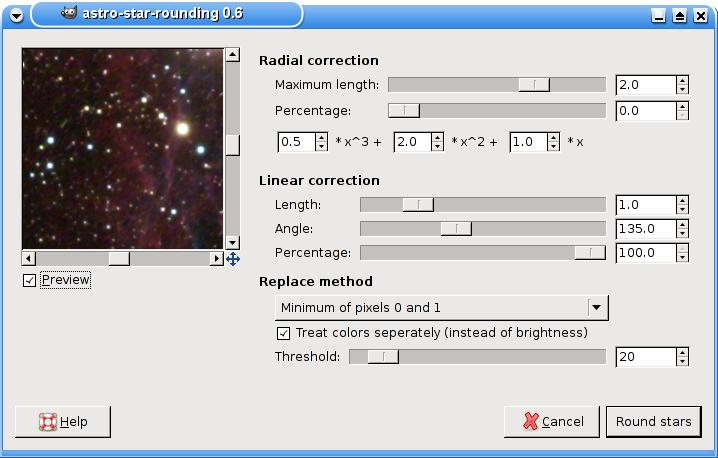
\includegraphics[width=0.8\textwidth]{star_rounding.jpg}\end{center}

\subsubsection{Usage}

This plugin can round stars, that are longish due to guiding errors or due to an uneven field (longish in radial direction).
The length values should match the elongation of the stars. The percentages determine, how much of the correction is applied.

Example:
\begin{multicols}{2}{
\begin{center}
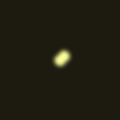
\includegraphics[width=0.3\textwidth]{star_rounding_long.png} \\
before
\end{center}

\begin{center}
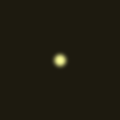
\includegraphics[width=0.3\textwidth]{star_rounding_rounded.png} \\
after
\end{center}
}\end{multicols}

\subsubsection{Explanation}

This plugin loops two times through all pixels of a drawable, either a complete layer or a selected area.

The first time, a radial elongation is corrected.
For this purpose, the length is calculated at each pixel, depending on the distance $r$ from the middle of the drawable, where the coefficients of the polynomial are given by the user:
$$P(r) = a_3 r^3 + a_2 r^2 + a_3 r$$
So in the middle, the length would be $0$, and in the corners the given maximum length.
The angle is calculated, depending on the position of the current pixel.

The second loop corrects a linear elongation with given length $L$ and angle $\phi$.

For each pixel, a minimum (or maximum) value is calculated, depending on length $L$ and angle $\phi$, either calculated for each pixel (radial correction) or constant (linear elongation).

The minimum (or maximum) values are calculated in the following way:

Decide, whether the brightness of the current pixel value is bigger than the threshold value (for minimum) or smaller (for maximum).

If it isn't, don't modify the current pixel.

Otherwise, identify the pixels 0 to 4 (0 is the current pixel, 1-4 are the pixels where the vector $(L,\phi)$ is pointing to:

\begin{center}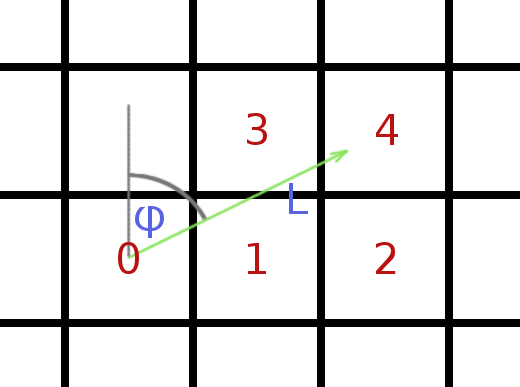
\includegraphics[width=0.5\textwidth]{star_rounding_drawing.png}\end{center}

Now, it calculates the brightness for pixels 0-5, where brightness is the greyscale value or calculated from RGB by
$$I=0.30 \cdot R + 0.59 \cdot G + 0.11 \cdot B$$

Then the distance from the point the vector is pointing to to the rows of pixels 1 and 2, and pixels 3 and 4, and to the columns of pixels 1 and 3, and pixels 2 and 4 is calculated.
In this example:
$$D_{\mathrm{row\ 3, 4}} = 0.17$$
$$D_{\mathrm{row\ 1, 2}} = 0.83$$
$$D_{\mathrm{column\ 1, 3}} = 0.69$$
$$D_{\mathrm{column\ 2, 4}} = 0.31$$

And from these distances a weighting value
$$W = 1 - D$$

Now it finds the pixel closest to the vector, in this example $(L=1.9,\phi=64.2^\circ)$ it is pixel 4.

The new pixel value is now calculated from all these values in the following way, weighted by the given percentage value.
The result is either a color or greyscale value, or a brightness value not modifing the color:

\begin{itemize}

	\item \textbf{Minimum of pixels 0 and 1}
		$$\mathrm{R} = \mathrm{percentage} \cdot \mathrm{min}\{\mathrm{pixel\ 0,\ pixel\ closest\ to\ vector}\} + \left( 100 - \mathrm{percentage} \right) \cdot \mathrm{pixel\ 0}$$
		In our example:
		$$\mathrm{R} = \mathrm{percentage} \cdot \mathrm{min}\{\mathrm{pixel\ 0,\ pixel\ 4}\} + \left( 100 - \mathrm{percentage} \right) \cdot \mathrm{pixel\ 0}$$

	\item \textbf{Minimum of pixels 0-4}
		$$\mathrm{R} = \mathrm{percentage} \cdot \mathrm{min}\{\mathrm{pixel\ 0,\ pixel\ 1,\ pixel\ 2,\ pixel\ 3,\ pixel\ 4}\} + \left( 100 - \mathrm{percentage} \right) \cdot \mathrm{pixel\ 0}$$

	\item \textbf{Minimum of pixel 0 and mean value of pixels 1-4}
		$$\mathrm{R} = \mathrm{percentage} \cdot \mathrm{min}\{\mathrm{pixel\ 0,\ \sum_{i=1}^4 W_{row} \cdot W_{column} \cdot pixel\ i}\} + \left( 100 - \mathrm{percentage} \right) \cdot \mathrm{pixel\ 0}$$
		In our example:

		$\mathrm{R} = \mathrm{percentage} \cdot \mathrm{min}\{\mathrm{pixel\ 0,\ 0.17 \cdot 0.31 \cdot\ pixel\ 1\ +\ 0.17 \cdot 0.69 \cdot\ pixel\ 2\ }$ \\
		$\mathrm{+\ 0.83 \cdot 0.31 \cdot\ pixel\ 3\ +\ 0.83 \cdot 0.69 \cdot\ pixel\ 4}\} + \left( 100 - \mathrm{percentage} \right) \cdot \mathrm{pixel\ 0}$

	\item \textbf{Maximum of pixels 0 and 1}
		$$\mathrm{R} = \mathrm{percentage} \cdot \mathrm{max}\{\mathrm{pixel\ 0,\ pixel\ closest\ to\ vector}\} + \left( 100 - \mathrm{percentage} \right) \cdot \mathrm{pixel\ 0}$$
		In our example:
		$$\mathrm{R} = \mathrm{percentage} \cdot \mathrm{max}\{\mathrm{pixel\ 0,\ pixel\ 4}\} + \left( 100 - \mathrm{percentage} \right) \cdot \mathrm{pixel\ 0}$$

	\item \textbf{Maximum of pixels 0-4}
		$$\mathrm{R} = \mathrm{percentage} \cdot \mathrm{max}\{\mathrm{pixel\ 0,\ pixel\ 1,\ pixel\ 2,\ pixel\ 3,\ pixel\ 4}\} + \left( 100 - \mathrm{percentage} \right) \cdot \mathrm{pixel\ 0}$$

	\item \textbf{Maximum of pixel 0 and mean value of pixels 1-4}
		$$\mathrm{R} = \mathrm{percentage} \cdot \mathrm{max}\{\mathrm{pixel\ 0,\ \sum_{i=1}^4 W_{row} \cdot W_{column} \cdot pixel\ i}\} + \left( 100 - \mathrm{percentage} \right) \cdot \mathrm{pixel\ 0}$$
		In our example:

		$\mathrm{R} = \mathrm{percentage} \cdot \mathrm{max}\{\mathrm{pixel\ 0,\ 0.17 \cdot 0.31 \cdot\ pixel\ 1\ +\ 0.17 \cdot 0.69 \cdot\ pixel\ 2\ }$ \\
		$\mathrm{+\ 0.83 \cdot 0.31 \cdot\ pixel\ 3\ +\ 0.83 \cdot 0.69 \cdot\ pixel\ 4}\} + \left( 100 - \mathrm{percentage} \right) \cdot \mathrm{pixel\ 0}$

\end{itemize}

The result is written back to the drawable. The alpha channel is not modified.

\end{document}
